\documentclass[12pt]{article}
\usepackage{graphicx}
\usepackage{amsmath}
\usepackage{hyperref}
% \bibliographystyle{plain}
% \bibliography{references}

% Title and Author
\title{Nash Equilibrium: A Comprehensive Overview}
\author{{\Large Arnab Sarker \& Enayet Alvee} \\
2105099   \& 2105107     \\
Bangladesh University of Engineering and Technology}
\date{\today}

% Document
\begin{document}

\maketitle
\pagebreak

\begin{abstract}
Nash Equilibrium, a pivotal concept in game theory, provides insights into strategic decision-making where the actions of participants are interdependent. It represents situations where each participant chooses their best response, considering the choices of others, leading to a state where no player can unilaterally improve their outcome. This equilibrium concept is foundational in understanding the behaviors of rational agents in various interactive settings. From competitive markets and evolutionary biology to the optimization of artificial intelligence algorithms, the Nash Equilibrium framework proves invaluable. This report delves into its theoretical underpinnings, computational methods, and vast applications, ranging from economics and politics to technology and societal dynamics. By examining historical developments, practical scenarios, and modern computational approaches, this comprehensive overview highlights the enduring relevance, adaptability, and utility of Nash Equilibrium in both theoretical and real-world contexts.
\end{abstract}

\tableofcontents
\pagebreak

\section{Introduction}
\large Nash Equilibrium, introduced by John Nash in the mid-20th century, is a foundational concept in game theory \cite{nash1950}. It describes a state in multi-player games where no participant can benefit by changing their strategy while others keep theirs unchanged \cite{osborne1994}. This equilibrium represents a stable point in decision-making processes, providing insights into how rational agents behave in competitive, cooperative, and mixed-strategy environments. Nash's breakthrough resolved many theoretical challenges in analyzing interdependent decisions and introduced a unified way to predict outcomes in strategic interactions.

The concept not only applies to economics but also extends to diverse fields such as biology \cite{smith1982}, computer science \cite{shoham2008}, and social sciences \cite{myerson1991}. For example, in biology, Nash Equilibrium explains evolutionary strategies, such as the balance between predator-prey relationships or cooperation within species. In technology, it informs the design of multi-agent systems that require coordination and competition, such as autonomous vehicles or distributed networks.

John Nash's pioneering work earned him the Nobel Memorial Prize in Economic Sciences in 1994, cementing his legacy as a key figure in game theory. This recognition reflects the profound implications of his work, not only for theoretical research but also for practical applications that influence various domains of modern life.

\section{Motivation}
\large The motivation to study Nash Equilibrium stems from its ability to model and predict behaviors in scenarios involving strategic interactions. As systems become more interconnected and decision-making increasingly complex, understanding equilibrium behavior becomes essential. Real-world applications demonstrate its wide-reaching significance:
\begin{itemize}
    \item \textbf{Economic Markets:} Understanding pricing strategies and market stability in competitive industries \cite{klemperer2002}. For instance, firms competing in an oligopolistic market often adjust their strategies to achieve equilibrium, ensuring profitability while maintaining competitive positioning.
    \item \textbf{Political Campaigns:} Analyzing voting strategies and alliances among political candidates \cite{feddersen1993}. By applying Nash Equilibrium, political parties can identify stable coalitions and optimize resource allocation to maximize voter support.
    \item \textbf{Biological Systems:} Exploring strategies in species interactions, such as cooperation and competition \cite{maynard1982}. Evolutionary game theory uses Nash Equilibrium to predict stable states in ecosystems, such as the coexistence of competing species or mutualistic relationships.
    \item \textbf{Technology and AI:} Developing algorithms for autonomous decision-making in multi-agent systems \cite{russell2020}. In robotics and artificial intelligence, equilibrium concepts guide the design of adaptive systems capable of functioning effectively in dynamic and competitive environments.
\end{itemize}

\begin{figure}[h!]
\centering
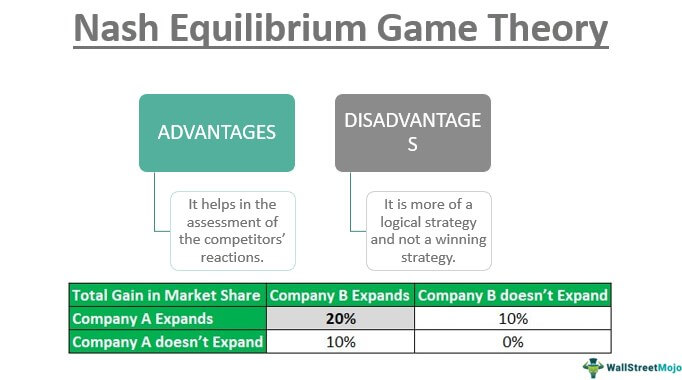
\includegraphics[width=0.8\textwidth]{Image/Nash-Equilibrium-Game-Theory.jpg}
\caption{Illustration of Nash Equilibrium in a Two-Player Game.}
\label{fig:nash_equilibrium}
\end{figure}

Studying Nash Equilibrium provides a structured way to navigate complex decision-making landscapes, offering insights into stable and optimal strategies. This makes it a critical tool for addressing challenges in resource allocation, policy formulation, and technological development.

\section{Algorithms}
\subsection{\texorpdfstring{$\frac{3}{4}$}{3/4}-Nash Equilibrium}

    Consider any positively normalized $n \times m$ bimatrix game $\Gamma=(A,B)$ and let $a_{i_1,j_1} = \max_{i,j}a_{i,j}$ and $b_{i_2,j_2} = \max_{i,j}b_{i,j}$. Then the pair of strategies $(\hat{x},\hat{y})$ where $\hat{x}_{i_1}=\hat{x}_{i_2}=\hat{y}_{i_1}=\hat{y}_{i_2}=\frac{1}{2}$ is a $\frac{3}{4}$-Nash Equilibrium for $\Gamma$.




    First, observe the expected payoff for player 1:
    \begin{align*}
        \hat{x}^T A \hat{y} &= \sum_{i=1}^n \sum_{j=1}^m \hat{x}_i \hat{y}_j a_{i,j} \\
        &= \hat{x}_{i_1} \hat{y}_{j_1} a_{i_1,j_1} +  \hat{x}_{i_1} \hat{y}_{j_2} a_{i_1,j_2} +  \hat{x}_{i_2} \hat{y}_{j_1} a_{i_2,j_1} +  \hat{x}_{i_2} \hat{y}_{j_2} a_{i_2,j_2} \\
        &= \frac{1}{4}(a_{i_1,j_1} + a_{i_1,j_2} + a_{i_2,j_1} + a_{i_2,j_2}) \\
        &\geq \frac{1}{4} a_{i_1,j_1}.
    \end{align*}
    Similarly, for player 2:
    \begin{align*}
        \hat{x}^T B \hat{y} &= \sum_{i=1}^n \sum_{j=1}^m \hat{x}_i \hat{y}_j b_{i,j} \\
        &= \hat{x}_{i_1} \hat{y}_{j_1} b_{i_1,j_1} +  \hat{x}_{i_1} \hat{y}_{j_2} b_{i_1,j_2} +  \hat{x}_{i_2} \hat{y}_{j_1} b_{i_2,j_1} +  \hat{x}_{i_2} \hat{y}_{j_2} b_{i_2,j_2} \\
        &= \frac{1}{4}(b_{i_1,j_1} + b_{i_1,j_2} + b_{i_2,j_1} + b_{i_2,j_2}) \\
        &\geq \frac{1}{4} b_{i_1,j_1}.
    \end{align*}
\pagebreak
\subsection{Metaheuristic Algorithms}
    \begin{table}[ht]
    \centering
    \caption{Metaheuristics Algorithms Summarized}
    \begin{tabular}{|p{3cm}|p{8cm}|p{3cm}|}
    \hline
    \textbf{Algorithm Name} & \textbf{Short Description} & \textbf{Per Iteration Complexity} \\
    \hline
    \textbf{Replicator Dynamics} & Evolutionary algorithm where players' strategies evolve over time based on payoff ratios, imitating more successful strategies. & $O(N^2)$ \\
    \hline
    \textbf{Particle Swarm Optimization (PSO)} & Population-based optimization algorithm where particles represent strategy profiles. They iteratively update based on personal and global best solutions. & $O(PNK)$ \\
    \hline
    \textbf{Simulated Annealing (SA)} & A single-point optimization technique that probabilistically explores the strategy space, reducing the search range over time. & $O(NK)$ \\
    \hline
    \end{tabular}
    \end{table}


\subsection{Heuristic Algorithms}
\begin{table}[ht]
\centering
\caption{Heuristic Algorithms Summarized}
\begin{tabular}{|p{3cm}|p{8cm}|p{3cm}|}
\hline
\textbf{Algorithm Name} & \textbf{Short Description} & \textbf{Per Iteration Complexity} \\
\hline
\textbf{Local Search} & Iteratively improves a solution by exploring neighboring solutions and accepting better ones. & $O(NK)$ \\
\hline
\textbf{Best Response Dynamics} & Players iteratively choose their best response (greedy choice) given the current strategies of others. & $O(NK)$ \\
\hline
\textbf{Hill Climbing} & A greedy algorithm that moves to the best neighboring solution, but may get stuck in local optima. & $O(NK)$ \\
\hline
\end{tabular}
\end{table}

\section{Applications}
\large Nash Equilibrium finds practical utility across various domains:
\begin{itemize}
    \item \textbf{Economics:} Pricing strategies in oligopolistic markets, ensuring stability amidst competition \cite{klemperer2002}. For example, companies like Apple and Samsung engage in strategic decision-making regarding product pricing, advertising, and innovation to maintain market equilibrium.
    \item \textbf{Social Media:} Algorithms to optimize content visibility and user engagement \cite{shoham2008}. Social media platforms balance user preferences and content diversity to maintain engagement while ensuring equitable content distribution.
    \item \textbf{Healthcare:} Designing treatment plans that balance effectiveness and cost-efficiency \cite{myerson1991}. Nash Equilibrium can inform policies to allocate medical resources effectively during crises, such as pandemics.
    \item \textbf{Sports:} Strategy formulation in team games to counter opponents’ tactics effectively \cite{smith1982}. In sports like football or tennis, equilibrium strategies help teams and players anticipate opponents' actions and respond optimally.
    \item \textbf{Politics:} Crafting campaign strategies that stabilize voter support across different demographics \cite{feddersen1993}. By analyzing voter preferences and competition dynamics, Nash Equilibrium aids in forming robust political strategies.
    \item \textbf{Machine Learning:} Multi-agent systems training to achieve cooperative or competitive goals in simulated environments \cite{russell2020}. Game-theoretic principles enhance reinforcement learning in AI, particularly in adversarial and collaborative tasks.
    \item \textbf{Traffic Management:} Optimizing route selections to reduce congestion and improve efficiency \cite{papadimitriou2007}. Equilibrium-based algorithms guide traffic flow in urban areas, minimizing delays and enhancing overall transportation efficiency.
\end{itemize}

\begin{figure}[h!]
\centering
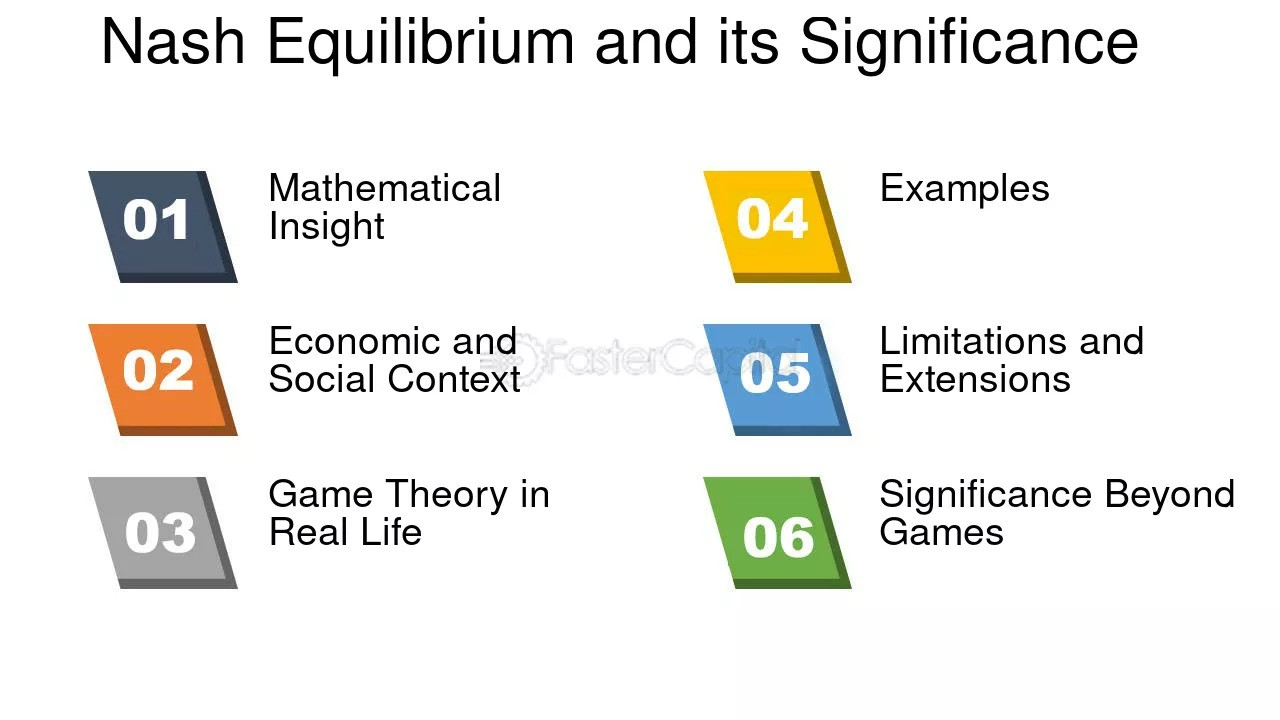
\includegraphics[width=0.8\textwidth]{Image/Example_nash-ezgif.com-webp-to-jpg-converter.jpg}
\caption{Illustration of Nash Equilibrium in a Two-Player Game.}
\label{fig:nash_equilibrium}
\end{figure}



The diverse applications of Nash Equilibrium underscore its adaptability and importance in solving real-world problems. From optimizing strategies in competitive markets to fostering cooperation in complex systems, this framework provides invaluable tools for decision-makers.

\section{Conclusion}
\large Nash Equilibrium offers a powerful lens to understand and predict outcomes in strategic interactions. Its interdisciplinary applications underscore its versatility and impact, making it a critical tool for decision-makers and researchers alike. By blending theoretical insights with computational advancements, Nash Equilibrium continues to shape our understanding of complex systems, fostering stability and innovation.

\section{References}
% \large \begin{enumerate}
%     \item Nash, J. F. (1950). "Equilibrium Points in N-Person Games." \textit{Proceedings of the National Academy of Sciences}. \label{nash1950}
%     \item Nash, J. F. (1951). "Non-Cooperative Games." \textit{Annals of Mathematics}. \label{nash1951}

%     \item von Neumann, J., \& Morgenstern, O. (1944). \textit{Theory of Games and Economic Behavior}. Princeton University Press. \label{vonNeumann1928}

%     \item Osborne, M. J., \& Rubinstein, A. (1994). \textit{A Course in Game Theory}. MIT Press. \label{osborne1994}

%     \item Maynard Smith, J. (1982). \textit{Evolution and the Theory of Games}. Cambridge University Press. \label{smith1982}

%     \item Myerson, R. B. (1991). \textit{Game Theory: Analysis of Conflict}. Harvard University Press. \label{myerson1991}

%     \item Shoham, Y., \& Leyton-Brown, K. (2008). \textit{Multiagent Systems: Algorithmic, Game-Theoretic, and Logical Foundations}. Cambridge University Press. \label{shoham2008}

%     \item Klemperer, P. (2002). "What Really Matters in Auction Design." \textit{Journal of Economic Perspectives}. \label{klemperer2002}

%     \item Papadimitriou, C. H. (2007). "The Complexity of Finding Nash Equilibria." \textit{Algorithmic Game Theory}. \label{papadimitriou2007}

%     \item Feddersen, T., \& Pesendorfer, W. (1993). "The Swing Voter's Curse." \textit{The American Economic Review}. \label{feddersen1993}

%     \item Russell, S., \& Norvig, P. (2020). \textit{Artificial Intelligence: A Modern Approach}. Pearson. \label{russell2020}
% \end{enumerate}

\footnotesize{
    \begin{thebibliography}{99}
        \bibitem{nash1950}
        Nash, J. F. (1950). "Equilibrium Points in N-Person Games." \textit{Proceedings of the National Academy of Sciences}.

        \bibitem{nash1951}
        Nash, J. F. (1951). "Non-Cooperative Games." \textit{Annals of Mathematics}.

        \bibitem{vonNeumann1928}
        von Neumann, J., \& Morgenstern, O. (1944). \textit{Theory of Games and Economic Behavior}. Princeton University Press.

        \bibitem{osborne1994}Osborne, M. J., \& Rubinstein, A. (1994). \textit{A Course in Game Theory}. MIT Press.

        \bibitem{smith1982}Maynard Smith, J. (1982). \textit{Evolution and the Theory of Games}. Cambridge University Press.

        \bibitem{myerson1991}Myerson, R. B. (1991). \textit{Game Theory: Analysis of Conflict}. Harvard University Press.

        \bibitem{shoham2008}Shoham, Y., \& Leyton-Brown, K. (2008). \textit{Multiagent Systems: Algorithmic, Game-Theoretic, and Logical Foundations}. Cambridge University Press.

        \bibitem{klemperer2002}Klemperer, P. (2002). "What Really Matters in Auction Design." \textit{Journal of Economic Perspectives}.

        \bibitem{papadimitriou2007}Papadimitriou, C. H. (2007). "The Complexity of Finding Nash Equilibria." \textit{Algorithmic Game Theory}. 

        \bibitem{feddersen1993}Feddersen, T., \& Pesendorfer, W. (1993). "The Swing Voter's Curse." \textit{The American Economic Review}.

        \bibitem{russell2020}Russell, S., \& Norvig, P. (2020). \textit{Artificial Intelligence: A Modern Approach}. Pearson
        \end{thebibliography}
   }     
        
\end{document}